\graphicspath{{chapters/09/images}}
\chapter{Gradient methods}
When we integrate to find ODE solutions, we do not obtain a function as
a solution, just points. In our optimization problem we do not know $f$ and $f'$(only sometimes
we do), so we are required to use \emph{numerical approximation}. The idea of
looking at $f'$ and set $f'=0$ is still at the base of gradient methods.
\\
\\
\noindent
If the problem contains constraints, how do we solve it? In this case
the problem is:

$$\left\{\begin{array}{ll}
\max f(x) &  \\
g_i(x)=0, & i \in \mathcal{I} \\
x \in \mathbb{R}^N
\end{array}\right.$$
\noindent
Let $\mathcal{I}= 1,...,m$. The traditional way to solve this problem is
to translate this system to another function. The Lagrangian function is
used to take into account the constraints.


\subsubsection{Lagrangian function}

We define the \textbf{\emph{Lagrangian function}} as
$L: \mathbb{R}^n \times \mathbb{R}^m \rightarrow \mathbb{R}$ s.t.

$$
L(x)= f(x) + \lambda g(x) = f(x) + \sum_{j=1}^m \lambda_j g_j(x)
$$


\subsection{Lagrangian Multipliers Theorem}

If $x^*$ is a stationary point for (Lagrangian function), then
$\exists \lambda^*$ s.t. $(x^* \lambda^*)$ is a stationary point for L. It
is a necessary condition (not sufficient, only one direction). This is a ``bigger'' problem, from
$\mathbb{R}^N \rightarrow \mathbb{R}^N \times \mathbb{R}^m$ . But still,
I can search solutions using stationary points. We can generalize the
idea to $g_i(x) \leq 0,$ constraints
\\
\\
\noindent
Remember that stationary points are not necessarily minima and maxima.
We check whether a stationary point is a max/min through second
derivations or evaluate the function in ``other'' points.

\subsection{Definition of a gradient}

Let $f: \mathbb{R}^N \rightarrow \mathbb{R}$ a differentiable function, we call gradient of $f$

$\nabla f: \mathbb{R}^N \rightarrow \mathbb{R}^N$ sit.
$\nabla f_i=\frac{\partial}{\partial x_i} f(x)_i$ and
$\nabla f(x) =\left[\begin{array}{c}\frac{\partial}{\partial x_1} f(x) \\ \vdots \\ \frac{y}{\partial x_N} f(x)\end{array}\right]$
\\
\\
\noindent
We look for points for which the derivative vanishes
$x^* : \nabla f(x^*)=0$
\\
\\
\noindent
TRY at home:$f(x, y)=(1-x)^2+100\left(y-x^2\right)^2 \\ f(x, y)=-(y+47) \sin \left(\sqrt{\left.\mid \frac{x}{2}+(y+47)\right|}-\right. x \cdot \sin \left(\sqrt{\left.\mid x-(y+47\right)|}\right).$
\\
\\
\noindent
These two functions are used to test optimization algorithms. The first
is \textbf{Rosenbrock's function,} the second the \textbf{Eggholder
function}. Solving analytically these problems is hard. We cannot apply gradient methods for stochastic simulations, since the
function is not continuous.


\subsection{Limitations of gradient descent methods}

One of the major limitations of these algorithms is that we are focusing
on local minima, we never know if the distance is minimum. Furthermore,
sometimes we want to optimize more variables and it might not be optimal
to perfectly fit the solution to both of them → trade-off.
\\
\\
\noindent
Figure \ref{fig:ex}: if we have an equality constraint we are only considering the points
meeting the boundary (red). In an inequality constraint, we consider
everything inside the red circle (yellow area). Generally, constraints
reduce our search space; the Lagrangian tells us that the minimum point
with some multipliers will give a solution of the Lagrangian, which is
one function. If we find the solutions, we do not know if they are
solutions of the original conditions, but they are ideal candidates that
can then be checked.

\begin{figure}
\centering
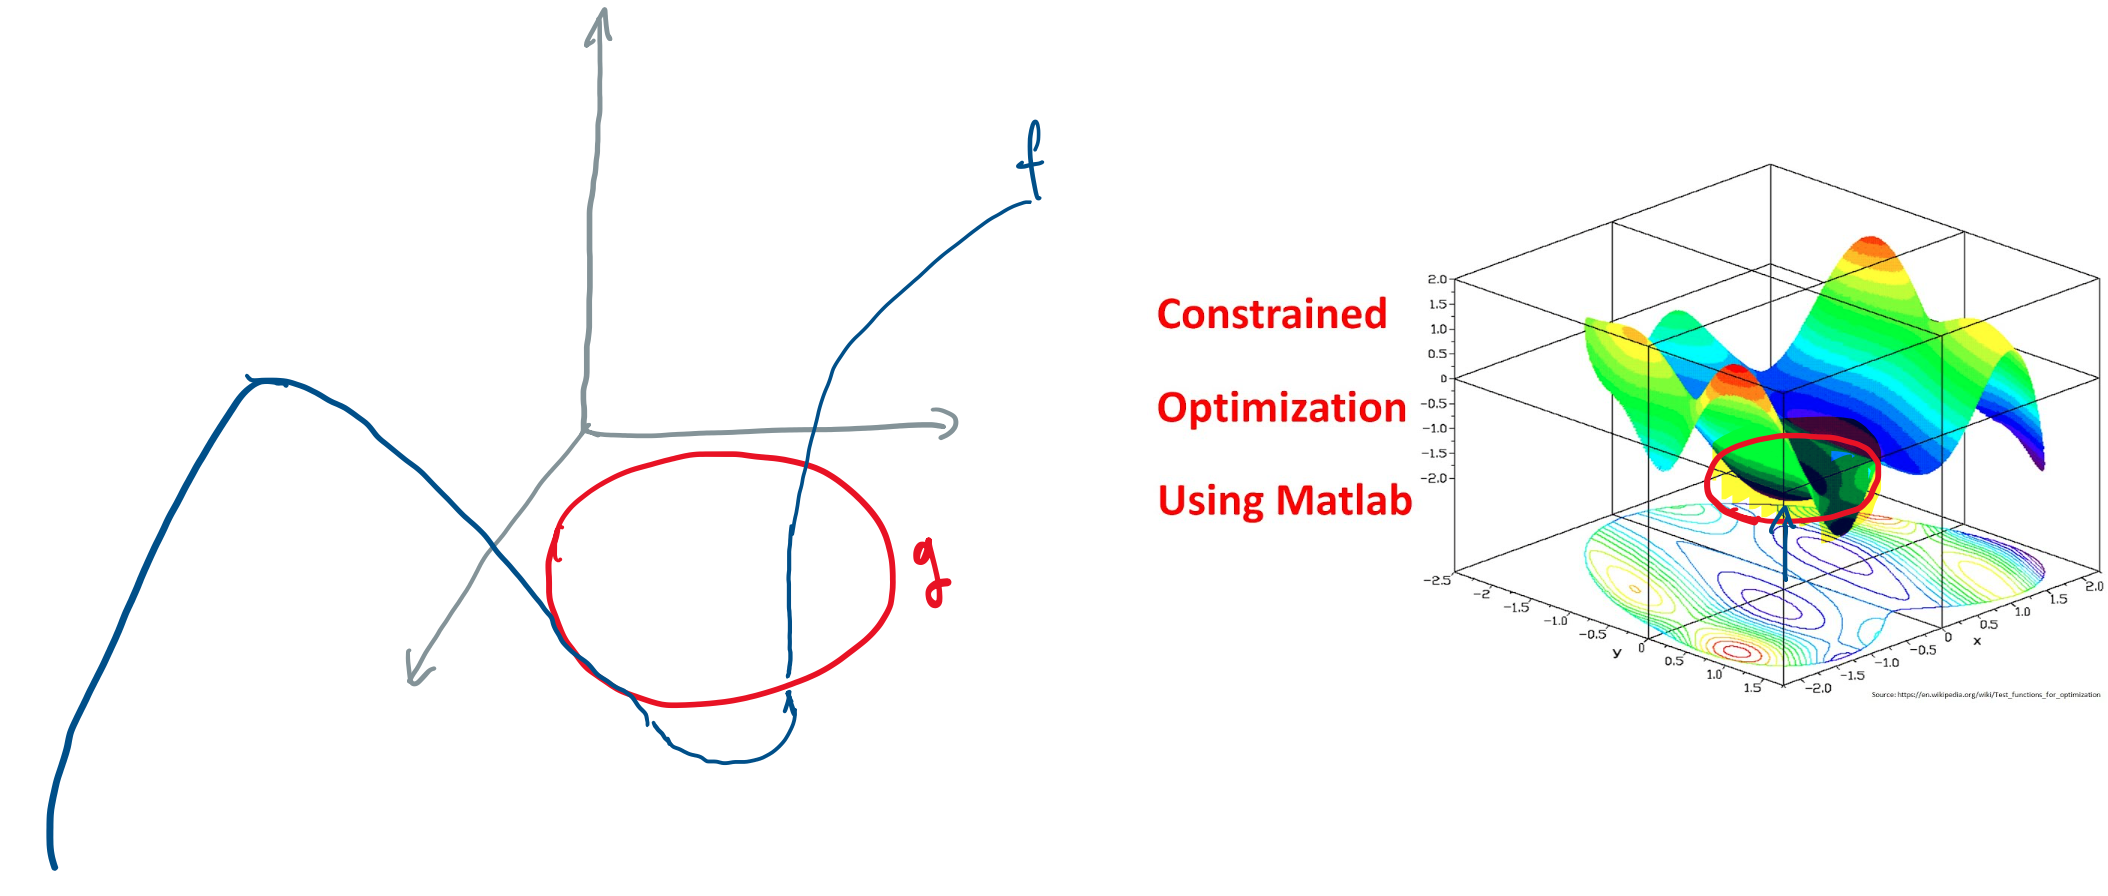
\includegraphics[width=0.5\textwidth]{example.png}
\caption{Blue = function, red = constraint}
\label{fig:ex}
\end{figure}
\noindent
For performing an evaluation of the distance we should integrate the
model, which is computationally expensive. To do one integration we must
perform a lot of computations. Our measure of computational cost is the
number of times we have to simulate the model (per iteration).
\\
\\
\noindent
In most cases, we do not know the gradient, therefore we should
approximate it using the Taylor formula.


\subsection{Gradient approximation with Taylor formula}

$(a,b) \in \mathbb{R}, x_0 \in (a,b)$
\\
\\
\noindent
Let $f_i(a,b) \rightarrow \mathbb{R}$ be differentiable $(n-1)$ times in
$(a,b)$ and $f^{(n)}$ is continuous in $x_0$. Then let $x \in (a,b)$ ,
we have:

$$
f(x)=f\left(x_0\right)+f^{\prime}\left(x_0\right)\left(x-x_0\right)+f''(x_0)\frac{(x-x_0)^2}{2!}+ ...+ f^{(n)}(x_0)\frac{(x-x_0)^n}{n!} + R_n(x) \text{ s.t.} \lim_{x \rightarrow x_0} \frac{R_n(x)}{(x-x_0)^n} =0
$$
\noindent
We focus on the first terms
$f(x)=f\left(x_0\right)+f^{\prime}\left(x_0\right)\left(x-x_0\right)+R_2(x)=0 \\ f^{\prime}\left(x_0\right)= \frac{f(x)-f(x_0)}{x-x_0}+\left(\frac{R_2(x)}{(x-x_0)}\right)=\frac{f(x)-f\left(x_0\right)}{x-x_0}+R_1(x).$
\\
\noindent
We can also use this trick for $N>1$
\\
\\
\noindent
Let $f: \mathbb{R}^N \rightarrow \mathbb{R}$ and
$e_i=(0, \ldots, 0,1,0,\ldots,0)$.
\noindent
Let's consider $x_1 x+\varepsilon e_i, x-\varepsilon e_i$ ; we are only
moving along one direction.
\noindent
In this case:
$$f\left(x+\varepsilon e_i\right)=f(x)+\varepsilon \frac{\partial f}{\partial x_i}(x)+\frac{1}{2} \varepsilon^2 \frac{\partial^2 f}{\partial x_i{ }^2}(x)+R_3(x) \\ f\left(x-\varepsilon e_i\right)=f(x)-\varepsilon \frac{\partial f}{\partial x_i}(x)+\frac{1}{2} \varepsilon^2 \frac{\partial^2 f}{\partial x_i{ }^2}(x)+R_3(x) \\ \Rightarrow f\left(x+\varepsilon e_i\right)-f\left(x-\varepsilon e_i\right)=+2 \varepsilon \frac{\partial f}{\partial x_i}(x)+R_3(x) \\ \Rightarrow \frac{\partial f}{\partial x_i}(x)=\frac{f\left(x+\varepsilon e_i\right)-f\left(x-\varepsilon e_i\right)}{2 \varepsilon}+R_2(x)$$
\noindent
We have computed an approximation of the first derivative with improved
accuracy.
\\
\\
\noindent
Consider that this only applies to one derivative, we have to perform
this at least twice → 2 function evaluation for each $i \Rightarrow 2W$.
In order to obtain a decent gradient, we require a lot of computations,
but they are fast (quite low number of iterations). We will see other
methods, which are somehow more precise, but also heavier.
\\
\\
\noindent
We can always check $\Delta f=0$ or not to understand if we are done!
\\
\\
\noindent
As we already saw, there might be points where the gradient vanishes
which are not the final destination. Gradient methods may tend to
overfitting, but they are effective. The main issue is that since we
approximate the gradient, we do not trust it everywhere.
\\
\\
\noindent
Gradient methods can be applied to two different categories of problems:

\begin{itemize}
\tightlist
\item
  constrained
\item
  unconstrained

  \begin{itemize}
  \tightlist
  \item
    \textbf{line search algorithm}: follow a direction
  \item
    \textbf{trust region:} create an approximation of the problem
    and solve it in a small trustable region
  \end{itemize}
\end{itemize}


\subsection{Line search}

\subsubsection{Newton's direction}

If we consider Taylor's formula and let $x_k$ be our starting point, let
$\alpha \in \mathbb{R}^+$ step length and $p$ our direction
($x_k, p \in R^n$). For $n=1$, we have:

$$
f(x_k+\alpha p)=f(x_k) + \alpha p f'(x_k) + \frac{\alpha^2p^2}{2} f''(x_k) + r(p^3)
$$
\noindent
For simplicity set $\alpha=1$ and truncate the formula:

$$
f(x_n+p)=f(x_n) + p f'(x_n) + \frac{p^2}{2} f''(x_n) = m_k(p)
$$

→ instead of minimizing the initial $f$, we minimize the simple
polynomial $m_k(p)$.
\noindent
From this equation we can get the direction
$p = -\frac{f'(x_k)}{f''(x_k)}$, which is called \emph{Newton direction}
(best direction). When $n>1$,
$p = -(\nabla^2 f(x_k))^{-1}\nabla f(x_k)$. Finding the inverse of a
matrix is ``a pain'', not straightforward; this is why we will try to
approximate this part.

\subsubsection{Line search algorithm for function minimization}

Set $k=0$ and guess an initial point $x_0$ WHILE $||\nabla f(x_k)||>0$

\begin{enumerate}
\def\labelenumi{\arabic{enumi}.}
\tightlist
\item
  compute $p_k=-(\nabla^2f(x_k))^{-1}\nabla f(x_k)$
\item
  select $\alpha_k$
\item
  update
  $x_{k+1}=x_k+\alpha_kp_k = x_k -\alpha_k(\nabla^2f(x_k))^{-1}\nabla f(x_k)$
\item
  $k=k+1$
\end{enumerate}
\noindent
We stop when the gradient is equal to zero, but we do not really have
zeroes in our computers; therefore, we must apply a threshold
$\varepsilon$.
\\
\\
\noindent
At each iteration we have some issues:

\begin{itemize}
\tightlist
\item
  sometimes we require approximation to compute the inverse of a matrix
\item
  it is computationally expensive to compute all these gradients
\end{itemize}
\noindent
Nevertheless, going in this direction is smart. We can try to tackle the hardest part, i.e.~$p_k$ computation, by
approximation.


\subsubsection{Quasi Newton's direction}

To avoid the computation of $\nabla^2 f$, we build iteratively a
different matrix $B_k$, such that
$B_{k+1}\cdot (x_{k+1}-x_k) = \nabla f(x_{k+1})-\nabla f(x_k)$
{[}condition for the matrix{]}
\\
\\
\noindent
We are approximating the second derivative as second of the gradient.
Since we are already computing the gradient, we exploit it to prevent
extra computations. The difference with respect to standard Newton
direction is the Hessian, which is not computed here.

\textbf{Quasi-Newton direction}:
$P_{k+1}=- \alpha B_{k+1}^{-1} \nabla f(x_k+1)$


\subsubsection{Steepest descent direction}

We proceed in the direction that reduces the gradient the most:

$$
p= -\alpha \frac{\nabla f}{||\nabla f||}
$$
\noindent
In this case we are completely ignoring the second derivative, we only
focus on the gradient computation. This method converges slowly with
respect to Newton and Quasi-Newton's direction.

\hypertarget{selecting-alpha}{%
\subsubsection{\texorpdfstring{Selecting
$\alpha$}{Selecting }}\label{selecting-alpha}}

Ideally, we want to define $\alpha$ s.t.

$$
\bar{\alpha}= \arg \min_{\alpha>0} f(x_k+\alpha p)
$$
\noindent
This is another optimization problem, ideal situation. To avoid solving
the optimization, we usually consider $\alpha$ that satisfies :

$$
f(x_k+\alpha p) \leq f(x_k) + c_1\alpha \nabla f(x_n)^T p_k, c_1 \in (0,1)
$$
\noindent
\textbf{Armijo condition:} the reduction should be proportional to
$\alpha$ and $\nabla f(x_n)^T p_k$.
\noindent
Sometimes thing fails because of parameter choice: it is crucial to
understand why functions fails and how parameters tuning can affect the
most crucial steps in the algorithms.


\subsubsection{Convergence of a method}

The order of convergence of a method (for us) is a constant $\ell$, such
that exists the limit:

$$
\lim_{k \rightarrow \infty  }\frac{||f(x_{k+1})-f(x^*)||}{||f(x_{k})-f(x^*)||^\ell} = L >0
$$

Where $x^*$ is the solution and the method converges.
\\
\\
\noindent
We compare the new iteration (numerator) to the old iteration
(denominator); the limit should go to zero, the exponent is the speed -
the higher the exponent $\ell$, the faster will the upper term go to
zero with respect to the bottom one i.e.~faster convergence. The higher
the exponent, the less iterations are required (in general). For the
methods that we have previously seen:

\begin{itemize}
\tightlist
\item
  steepest descent: $\ell=1$, linear convergence
\item
  quasi-Newton: $\ell \in (1,2)$, superlinear convergence
\item
  Newton: $\ell=2$, quadratic convergence
\end{itemize}

Example: $f(x)=x^4-8x^2+4$

\begin{figure}
\centering
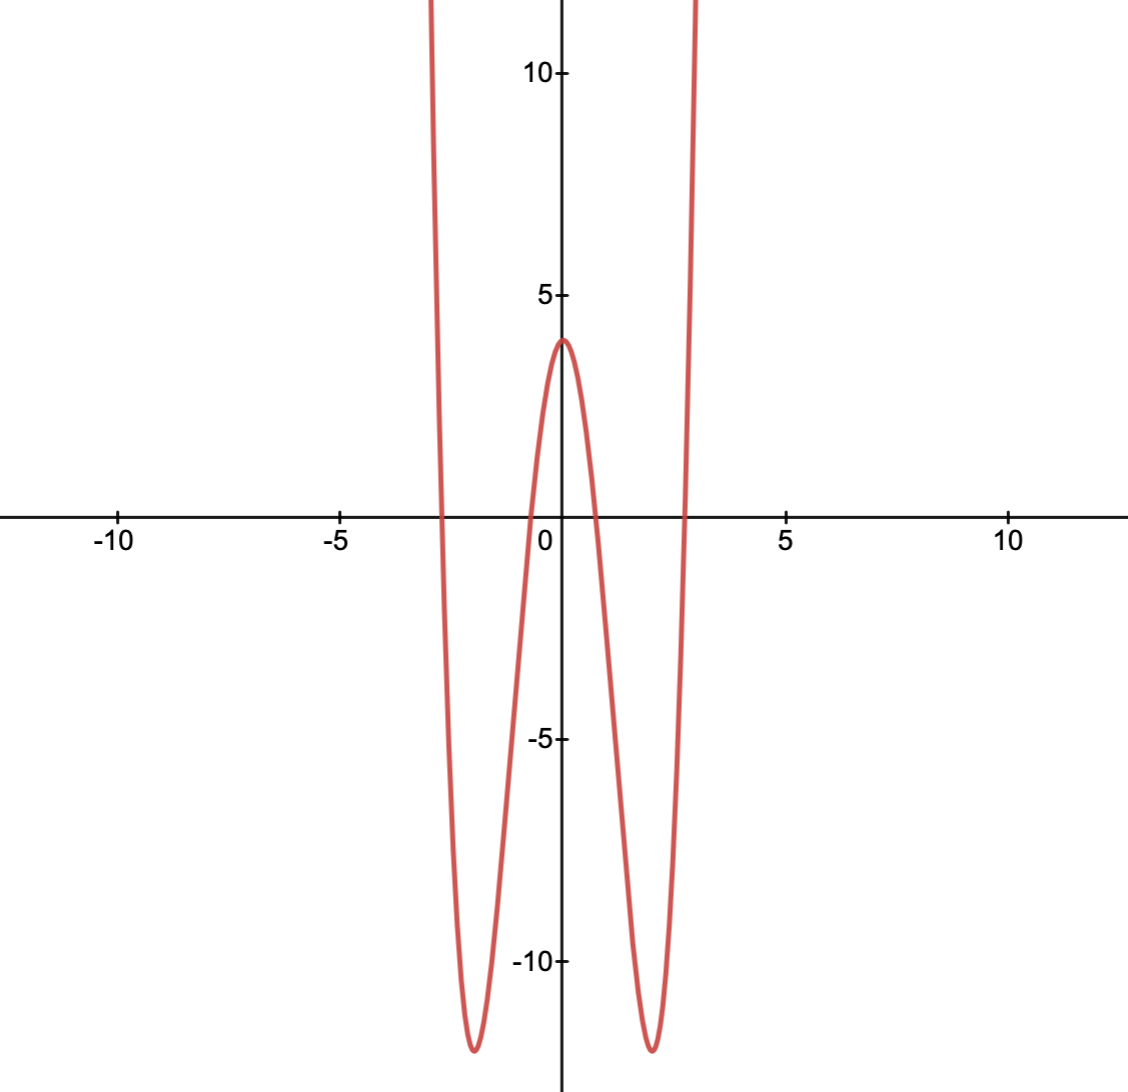
\includegraphics[width=0.3\textwidth]{function.png}
\caption{Desmos  $f(x)=x^4-8x^2+4$}
\end{figure}

$$
x_0=3 \\ f'(x) = 4x^3-16x \Rightarrow f'(x)=0 \Rightarrow  x=0, x=\pm 2\\ f''(x)=12x^2-16
$$

Algorithm: $f'(3)=60, f''(3)=92,$

Let $\alpha=1$:

$$
p_0= -\frac{60}{92}=-0.65 \\ x_1=3-0.65=2.35 \\ f'(2.35) = 14.31\\ f''(2.35) = 50.27 \\ p_1=-\frac{f'(x_1)}{f''(x_1)} = -0.28\\ x_2=x_1+\alpha p_1 = 2.35-0.28=2.07 \\ f'(x_2) = 2.30 \\ f''(x_2)=35.42\\ p_2 = -0.067
$$

Let's try the same by applying Steepest Descent method:

$f'(3)=60 \\ x_1 = x_0..$
$f'(3)=60$
\noindent
In this case the SDM is way faster, lucky shot. But what if we change
the starting point? The direction will always be the same,
i.e.~$p_1 = -1$.

$$
x_1=2.35-1=1.35\\f'(x_1)=-11.75\\x_2=1.35+1 = 2.35
$$

We are doing ping-pong among two points!
\\
\\
\noindent
The fact that the second derivative progressively shrinks tells us that
we need to reduce the step, but in this case we are not taking this into
account. Of course we also have $\alpha$, we should look at Armijo
condition and change it.
Take into account that each time that we are performing operation on a
number we lose precision.


\subsection{Trust region}

{[}picture{]}
\noindent
Imagine that this is a cut function: our starting point $x_k$ is in the
middle. The main idea of the trust region is that we do not follow a
direction: we approximate the function with a simpler function → Taylor
approximation. According to how big and reliable the approximation is,
we will choose a direction.
\\
\\
\noindent
Last time we approximated the model as:

$$
m(x_p+\alpha p)=f(x_k)+\alpha p^T \nabla f(x_k)+ \frac{1}{2} \alpha^2p^T B_k p
$$

$$
\alpha=1, m_k (p)=f_k+p^T\nabla f_k + \frac{1}{2} p^T B_k p
$$

\hypertarget{trust-region-steepest-descent}{%
\subsubsection{Trust region steepest
descent}\label{trust-region-steepest-descent}}

Define a region such that $||p|| < \delta_k,\delta_k>0$ in which we
solve the optimization problem (1) instead of the original. Remember
that $B_k$ can be the Hessian or an approximation; on the other hand, we
have said that we can also ignore it.
\\
\\
\noindent
Finding a minimum for $m_k(p)=f_k+p^T\nabla f_k$ means that we are
looking for:

$$
\min_p m_k(p)= \min_p (f_k+p^T\nabla f_k)
$$
\noindent
Remember that $f_k$ is a constant, so we want to find a direction for
which $\min_p p^T\nabla f_k$ is minimum. We can rewrite this as:

$$
p^T\nabla f_k = ||p|| ||\nabla f_k|| \cos \theta
$$
\noindent
We minimize for $p$ such that $\cos \theta = -1$ and $||p||=\delta_k$,
where p s.t. $||p|| \leq \delta_k$ {[}radius of the trust region{]}.

$$
\min_p p^T\nabla f_k = -\delta_k || \nabla f_k ||
$$

$$
p = - \delta_k \frac{\nabla f_k}{||\nabla f_k||}
$$
\noindent
This result is exactly the equation from steepest descent. We are
applying a condition on the region with $\delta_k$. This direction and
the whole approach is called trust region steepest descent.
\\
\\
\noindent
We could follow the same idea by applying Newton or Quasi-Newton.
\\
\\
\noindent
To evaluate if we can really trust our region, we define the
\textbf{\emph{actual reduction}} as:

$$
\rho_k = \frac{f(x_k)-f(x_k+p)}{m(x_k)-m(x_k+p)}
$$

By construction $m(x_k+p) \leq m(x_k)$.

\begin{itemize}
\tightlist
\item
  If $\rho_k < 0$ → reject $p$, we are not improving the real problem.
  Usually take $\delta_k = \frac{1}{4} \delta_k$
\item
  If $\rho_k \simeq 1$ → maybe longer step
\end{itemize}
\noindent
$\delta$ value can be tuned according to the needs. The approach is
similar to RK method seen with Marchetti. Of course we have a grey area
between 0 and 1, so we define a threshold e.g.~$\rho_k < \eta$ and
$\rho_k > \eta$.
\noindent
By default, MATLAB uses a trust region algorithm. Having something
certifying that we are doing good or bad is a great thing in
approximation!


\subsubsection{Trust region algorithm}

Let
$\hat{\delta}>0, \delta_0 \in (0,\hat{\delta}), \eta \in (0,\frac{1}{4})$

$k=0, \varepsilon < 0$

REPEAT

obtain $p_k \text{ s.t. } p_k=\arg \min_p m(x_k+p)$

compute $\rho_k$

IF $\rho_k < \frac{1}{4}$

$\delta_{k+1}=\frac{1}{4}\delta_k$

ELSEIF $(\rho_k < \frac{3}{4})$ AND $||p_k||=\delta_k$

$\delta_{k+1}=\min (2\delta_k, \hat{\delta})$

ELSE

$\delta_{k+1}=\delta_{k}$

IF $\rho_k > \eta$

$x_{k+1}= x_{k}+p_{k}$

ELSE

$x_{k+1}= x_{k}$

IF $||\nabla f(x_{k+1})||<0$

BREAK
\\
\\
\noindent
We stop if the gradient is sufficiently small. Our focus is on computing
$p_k$. We then evaluate $\rho_k$ to adjust parameters (which is simpler
from what we have previously seen).
\\
\\
\noindent
If we apply this algorithm to the example of last lecture, it happens
that with $x_0=235$ and steepest descent $\rho_0=0.17 < \frac{1}{4}$,
which tells us to reduce $\delta$. The only thing that changes is $\rho$
changes.
\\
\\
\noindent
PROBLEM:

$$
g(x,y)=x^4+y^4+xy
$$

\url{https://www.benfrederickson.com/numerical-optimization/} play with
learning rate, explore the site.
